\documentclass[twoside]{ctuthesis}

\ctusetup{
	mainlanguage = english,
	titlelanguage = english,
	otherlanguages = {czech,english},
	title-czech = {Vývoj RC auta řízeného pomocí STM32 microkontrolerů},
	title-english = {Development of RC car controlled by STM32 microcontrollers},
	doctype = B,
	faculty = F3,
	department-czech = {Katedra elektrických pohonů a trakce},
	department-english = {Department of Electric Drives and Traction},
	author = {Kristián Šlehofer},
	supervisor = {Ing. Jan Stejskal},
	supervisor-address = {Technická 1902/2,\\ Praha 6 \\ room: E1-107},
	keywords-czech = {}, 	%TODO
	keywords-english = {},	%TODO
	day = 14,				%TODO
	month = 1,				%TODO
	year = 2022,				%TODO
	%specification-file = {figs/zadani.pdf}, %TODO
	%department-czech = {Kybernetika a robotika},
	%department-english = {Cybernetics and robotics},
	%front-specification=true,
	front-list-of-figures=true, 
	front-list-of-tables=true
}

\ctuprocess

\addto\ctucaptionsczech{%
	\def\supervisorname{Vedoucí}%
	\def\subfieldofstudyname{Studijní program}%
}

\ctutemplateset{maketitle twocolumn default}{
	\begin{twocolumnfrontmatterpage}
		\ctutemplate{twocolumn.thanks}
		\ctutemplate{twocolumn.declaration}
		\ctutemplate{twocolumn.abstract.in.titlelanguage}
		\ctutemplate{twocolumn.abstract.in.secondlanguage}
		\ctutemplate{twocolumn.tableofcontents}
		\ctutemplate{twocolumn.listoffigures}
	\end{twocolumnfrontmatterpage}
}

% Theorem declarations, this is the reasonable default, anybody can do what they wish.
% If you prefer theorems in italics rather than slanted, use \theoremstyle{plainit}
\theoremstyle{plain}
\newtheorem{theorem}{Theorem}[chapter]
\newtheorem{corollary}[theorem]{Corollary}
\newtheorem{lemma}[theorem]{Lemma}
\newtheorem{proposition}[theorem]{Proposition}

\theoremstyle{definition}
\newtheorem{definition}[theorem]{Definition}
\newtheorem{example}[theorem]{Example}
\newtheorem{conjecture}[theorem]{Conjecture}

\theoremstyle{note}
\newtheorem*{remark*}{Remark}
\newtheorem{remark}[theorem]{Remark}

\setlength{\parskip}{5ex plus 0.2ex minus 0.2ex}



% Abstract in Czech
\begin{abstract-czech}
%TODO
\end{abstract-czech}

% Abstract in English
\begin{abstract-english}
%TODO
\end{abstract-english}

% Acknowledgements / Podekovani
\begin{thanks}
%TODO
\end{thanks}

% Declaration / Prohlaseni
\begin{declaration}
  %TODO

\end{declaration}

% Only for testing purposes
\listfiles


\usepackage[pagewise]{lineno}
\usepackage{lipsum,blindtext}
\usepackage{mathrsfs} % provides \mathscr used in the ridiculous examples
\usepackage{amsmath}
\usepackage{subcaption}
\DeclareMathOperator{\atantwo}{atan2}
\usepackage{float} 



\usepackage{hyperref}
\hypersetup{
	pdftitle={STM32 RC car},
	pdfauthor={Kristian Slehofer}
}

\usepackage{adjustbox}
\usepackage{verbatim}
\usepackage{tablefootnote} % for table footnotes

\usepackage{xurl}	% for too long urls
\usepackage{siunitx}	


\begin{document}
\maketitle



%!TEX ROOT=slehokri_bp.tex

\chapter{Introduction}
\label{chap:intro}
%TODO

\section{Motivation}
%TODO






%!TEX ROOT=main.tex


\part{STM32 microcontrollers}
\label{chap:STM}
\section{Indroduction}
\label{sec:stm_intro}
STM32 is a family of 32-bit microcontrollers by STMicroelectronics based on ARM Cortex-M processor, namely Cortex-M3, Cortex-M4(F), Cortex-M0, Cortex-M0+, Cortex-M7F, and Cortex-M33F. The STM32 family consists of numerous series of microcontrollers designed for various use-cases. These can be divided into four main groups: Mainstream, High Performance, Ultra-low-power, and Wireless series. As every series has specific features and peripherals, this section will only focus on the main differences between used ARM Cortex cores. Table \ref{tab:cortex} shows the utilization of ARM cores in the particular STM32 series.
%\begin{table}[ht]
%\begin{ctucolortab}
%\begin{tabular}{cc}
%\bfseries ARM Core & \bfseries STM32 series \\\Midrule
%Cortex-M3 & F1, F2, L1 \\ 
%Cortex-M4F & F3, F4, G4, L4, L4+, WB, WL\tablefootnote{Based only on ARM Cortex-M4 (without FPU).} \\	
%Cortex-M0 & F0 \\ 
%Cortex-M0+ & G0, L0 \\
%Cortex-M7F & F7, H7 \\
%Cortex-M33F & L5, U5
%\end{tabular}
%\end{ctucolortab}
%\caption{ARM Core utilization in STM32 family}
%\label{tab:cortex}
%\end{table}

\begin{table}[ht]
   \renewcommand{\arraystretch}{1.1}
   \centering
    \caption{ARM Core utilization in STM32 family}\label{tab:cortex}   
    \begin{tabular}{c c}
       \noalign{\hrule height 1.1pt}\noalign{\smallskip}
	   \bfseries ARM Core & \bfseries STM32 series\\[0.2em]
	\noalign{\hrule height 1.1pt}\noalign{\smallskip}     
Cortex-M3 & F1, F2, L1 \\ 
Cortex-M4F & F3, F4, G4, L4, L4+, WB, WL\tablefootnote{Based only on ARM Cortex-M4 (without FPU).} \\	
Cortex-M0 & F0 \\ 
Cortex-M0+ & G0, L0 \\
Cortex-M7F & F7, H7 \\
Cortex-M33F & L5, U5 \\
       \noalign{\smallskip}\noalign{\hrule height 1.1pt}
    \end{tabular}
\end{table} 

\section{Division by ARM cores}
\label{sec:stm_arm_division}
	\subsection{Cortex-M3}
	\label{sub:stm_m3}
Cortex-M3 was the first processor in the Cortex-M generation and the first core used in the STM32 family in the STM32F1 series of microcontrollers. ARM first released this high-performance processor based on ARMv7-M architecture in 2005. It features modified Harvard architecture (with unified memory space) and a 3-stage pipeline. Thanks to 32-bit addressing, 4GB of memory space is supported.
	
	\subsection{Cortex-M4F}
	\label{sub:stm_m4}
The successor to Cortex-M3 was released by ARM in 2010. This new generation called Cortex-M4 is similar to its predecessor in design and features. The instruction set now contains DSP (Digital Signal Processor) instructions for more complex data processing, and there is an optional single-precision FPU (Floating Point Unit). Variant with FPU is known as Cortex-M4F. 
	
	\subsection{Cortex-M0}
	\label{sub:stm_m0}		%TODO citace?
Cortex-M0 processor is one of the smallest ARM processors available, optimized for small size and low power consumption \cite{m0_web}. The processor is based on ARMv6-M with a smaller instruction set, uses Von Neumann architecture, and has a 3-stage pipeline. This small core is ideal for general data processing tasks, where low cost and high energy efficiency matter.
	
	\subsection{Cortex-M0+}
	\label{sub:stm_m0_plus}
Cortex-M0+ is based on Cortex-M0, thus adopting small a size and further improving power efficiency and performance. The instruction set and tools are fully backward compatible with Cortex-M0. ARM reduced pipeline to 2 stages to lower power consumption. Furthermore, the processor has more options available, such as vector table relocation and memory protection unit (MPU).
	
	\subsection{Cortex-M7F}
	\label{sub:stm_m7}
The most powerful processor in the Cortex-M family is Cortex-M7. The processor uses ARMv7-M architecture and features the longest pipeline with six stages. Given the used architecture, the instruction set contains DSP instructions, and there is also an optional FPU, which can be single-precision or even double-precision. Main buses have been enlarged to 64-bit wide. Variant with FPU is known as Cortex-M7F. 
	
	\subsection{Cortex-M33F}
	\label{sub:stm_m33}
Cortex-M33 is the newest core used in the STM32 family of microcontrollers. The processor is based on more recent ARMv8-M architecture with Harvard bus architecture. It is conceptually similar to Cortex-M4 with a 3-stage pipeline and optional single-precision FPU. The core is ideal for IoT applications as it has optional TrustZone security instructions for hardware-enforced isolation and memory protection unit (MPU). Variant with FPU is known as Cortex-M33F. 

\section{Architecture}
\label{sec:stm_arch}
ARM as a company does not construct microcontrollers but instead designs the core and other components and licenses them to silicon designers. It is the same concept with the STM32 family of microcontrollers - ST Microelectronics obtains the processor design from ARM as a base for their microcontroller. The company then attaches its own set of memories and peripherals, such as ADC (Analog-to-Digital converter), DAC (Digital-to-Analog converter), clock generation and timers, and various types of connectivity peripherals like UART, SPI, I2C, etc.

This approach is illustrated in figure \ref{fig:f303}, which shows the circuit diagram of the STM32F303CC microcontroller used in this project. It shows the Cortex-M4F processor with all the ST-specific peripherals and memories around.
\begin{figure}
\centering
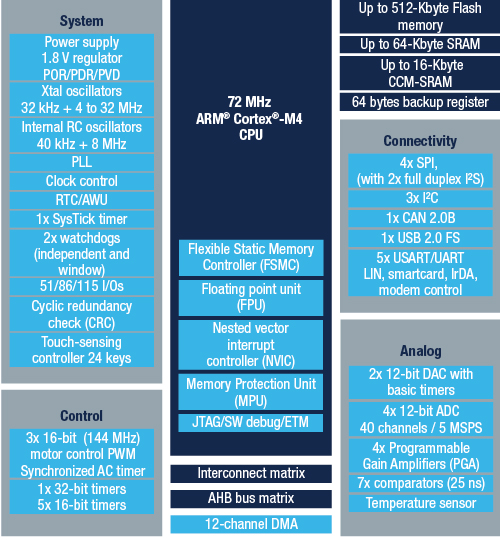
\includegraphics[width=0.6\linewidth]{support/pic/en.bd_stm32f303.jpg}
\caption{STM32F303 circuit diagram \cite{f303_diagram}} %TODO citace - web ST
\label{fig:f303}
\end{figure}

	\subsection{Clock}
	\label{sub:clock}
The frequency of the processor, buses, and connected peripherals is derived from their clock source, usually an oscillator. STM32 microcontrollers include internal clock sources, or it is possible to connect external clock sources. The frequency from other clock sources can be multiplied by the internal PLL (Phase-Locked Loop) circuit to speed up the microcontroller further and reach higher frequencies. Several prescalers allow finetuning bus and peripherals speed. Internal clock sources have the advantage of providing a clock source at a low cost with no external components. However, being an RC oscillator, the frequency produced is usually not as accurate as an external oscillator.

	\subsection{Interrupts}
	\label{sub:nvic}
The main controller responsible for handling interrupt events is Nested Vectored Interrupt Controller, NVIC for short. It is tightly coupled to the Cortex core allowing for low latency interrupt processing. The NVIC features support for up to 240 interrupt inputs with programmable priorities, which can be individually enabled or disabled, along with Non-Maskable Interrupts (NMI). Furthermore, in the case of Cortex M3 and M4, the interrupt latency is only 12 cycles with zero wait state memory \cite{yu}. All interrupts can be triggered by software by writing to the appropriate register; this also applies to many system exceptions. Microcontroller vendors determine the total number of interrupts supported by the device with Cortex core when designing the chip.

In the  STM32 family of microcontrollers, there is also a hardware device called extended interrupts and events controller (EXTI). This controller is connected to the NVIC and supports up to 36 external/internal interrupt events. Active edge for external interrupts is programmable. This device makes it possible to generate interrupts or wake-up events from external peripherals and GPIO pins.

	\subsection{Buses}
	\label{sub:buses}
The Cortex core has a well-defined on-chip bus structure and protocol that allows the connection of various memory configurations and peripherals. Since most of the Cortex cores use Harvard architecture, multiple bus interfaces enable simultaneous access to instructions and data. Buses are (most of the time) 32-bit wide.

The primary bus interface protocol utilized is AHB Lite (Advanced High-performance Bus). This pipelined protocol allows high operation frequency with a small silicon footprint and is used in program memory and system bus interfaces. Usually, the bus can have more devices that act as a master, for example, DMA (Direct Memory Acces) or Ethernet controller. Therefore the processor includes a bus matrix (or AHB interconnect matrix) that manages transfers from multiple bus masters to different slave segments. Particular bus matrix implementation is shown in figure \ref{fig:f303_busmatrix}.
\begin{figure}
\centering
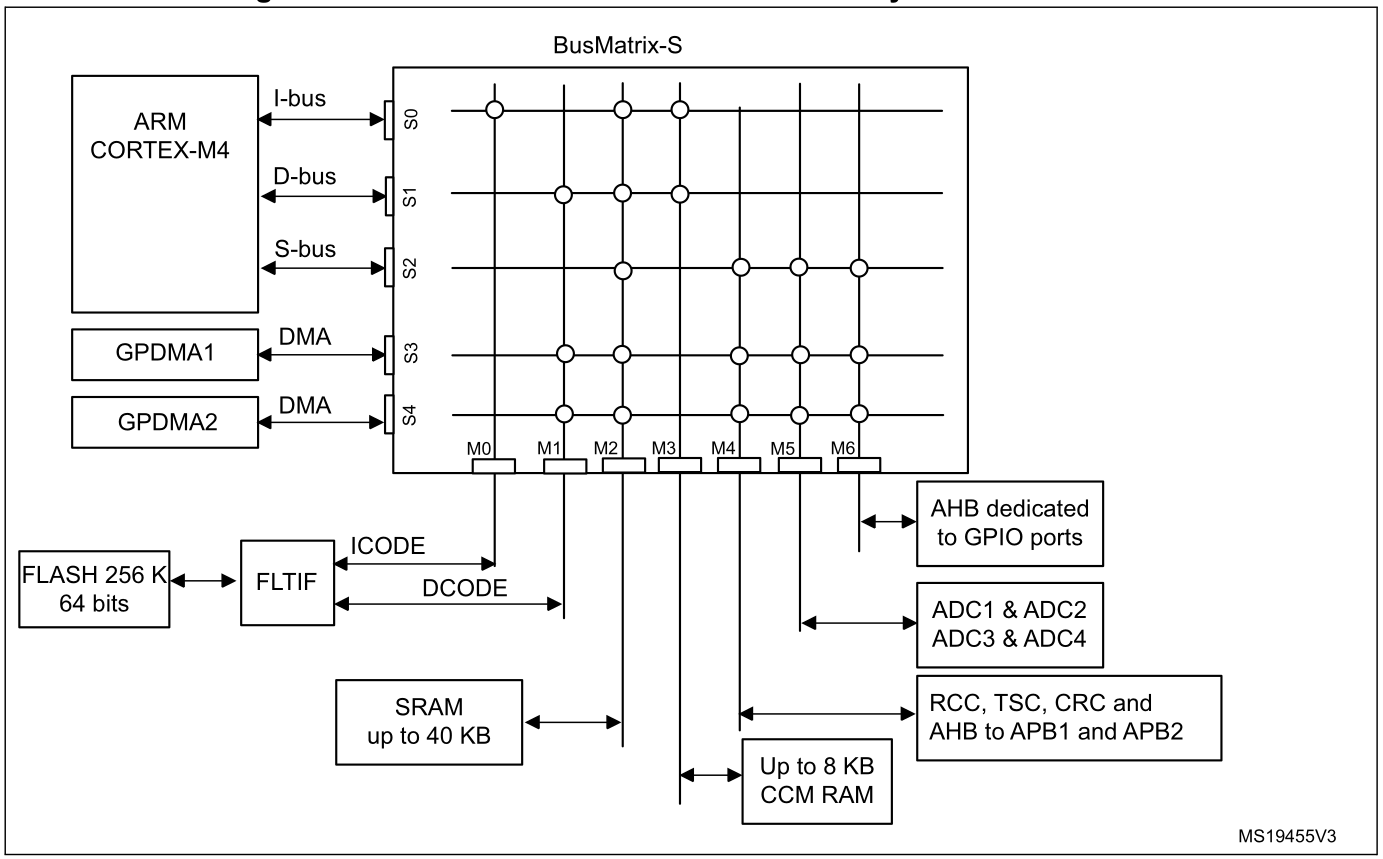
\includegraphics[width=0.7\linewidth]{support/pic/f303_bus_matrix.png}
\caption{STM32F303CC bus architecture \cite{f303_ref}} %TODO citace - referencak F303
\label{fig:f303_busmatrix}
\end{figure}

The secondary bus used mainly for connecting peripherals is APB (Advanced Peripheral Bus). Usually, APB buses are connected to the AHB bus matrix using bridge components. If the peripheral needs higher bandwidth and operation speed, for example, the ADC, it is possible to connect it to the faster AHB bus.

Some of the more advanced Cortex processors also use other buses. For example, the Cortex-M7 has an additional 64-bit wide AXI bus that can be used for faster FLASH memory access. 

	\subsection{Memories}
	\label{sub:memories}
Thanks to the bus architecture, different memories can easily be attached to the AHB bus with suitable memory interface logic. Even though the bus is 32-bit, there are no width restrictions if appropriate conversion hardware is used.

Usually, types like SRAM and FLASH are often used for data memory and program code memory, respectively. However, there is no real limitation on memory type connected to a processor, and different technologies can be utilized, e.g., SDRAM, EPROM, etc. Also, memory size is not limited. The only requirement is that the memory should be byte-addressable, and the interface has to support byte, half-word, and word transfers.

	\subsection{Direct Memory Acces (DMA)}
	\label{sub:dma}
A Direct Memory Access is a programmable hardware unit connected to the AHB bus. It reduces processor load by offloading memory transfer operations. Supported transfer directions are peripheral-to-peripheral, memory-to-peripheral, peripheral-to-memory, and also memory-to-memory. There is a small overhead when setting the unit, but afterward, the whole transfer is handled by DMA without processor intervention, thus leaving computing power to other tasks. The unit usually has several independent channels with assignable priorities.


\section{Peripherals}
\label{sec:stm_periph}
Every series of STM32 microcontrollers features different peripherals, from the basic ones with little settings to more advanced and configurable ones. This section is not supposed to be an overly exhausting listing of all the peripherals across all STM32 families, but instead, it focuses mainly on the most used ones and those used in this project.

	\subsection{GPIO}
	\label{sub:gpio}
The abbreviation GPIO stands for General-Purpose Input/Output. It is a designation for microcontroller pins. The pins are arranged in groups of sixteen and are referred to as GPIOx (for example, GPIOA, GPIOC). Not every pin from the group has to be physically present. Especially for microcontrollers with smaller packages, it is usual that some pins from the group are missing. In figure \ref{fig:gpio}, there is a typical internal structure of the GPIO pin with internal protection diodes.

Each pin can be set as either input, output, or alternate function. Internal pull-up and pull-down resistors are available as well. These features are configured and controlled by software. Most GPIO control registers are 32-bit and have to be accessed as 32-bit words, although some STM32 series support half-word and byte access.

If the pin is in alternate function mode, it is controlled by a connected peripheral, for example, ADC, timer, or USART. Thanks to the highly flexible pin multiplexing, many peripheral functions can be remapped to another pin. Debug pins are in alternate function mode by default after microcontroller reset. Other pins are usually in floating input mode.

When the pin is set as output or alternate function, it can be push-pull or open-drain. Most of the pins can provide $\pm20 \text{ mA}$ of current, making it possible to drive, for example, a LED directly. However, the total current that a microcontroller can source or sink is limited. Connecting pins to voltages higher than the supply voltage is not recommended, yet many pins are 5V tolerant.
\begin{figure}
\centering
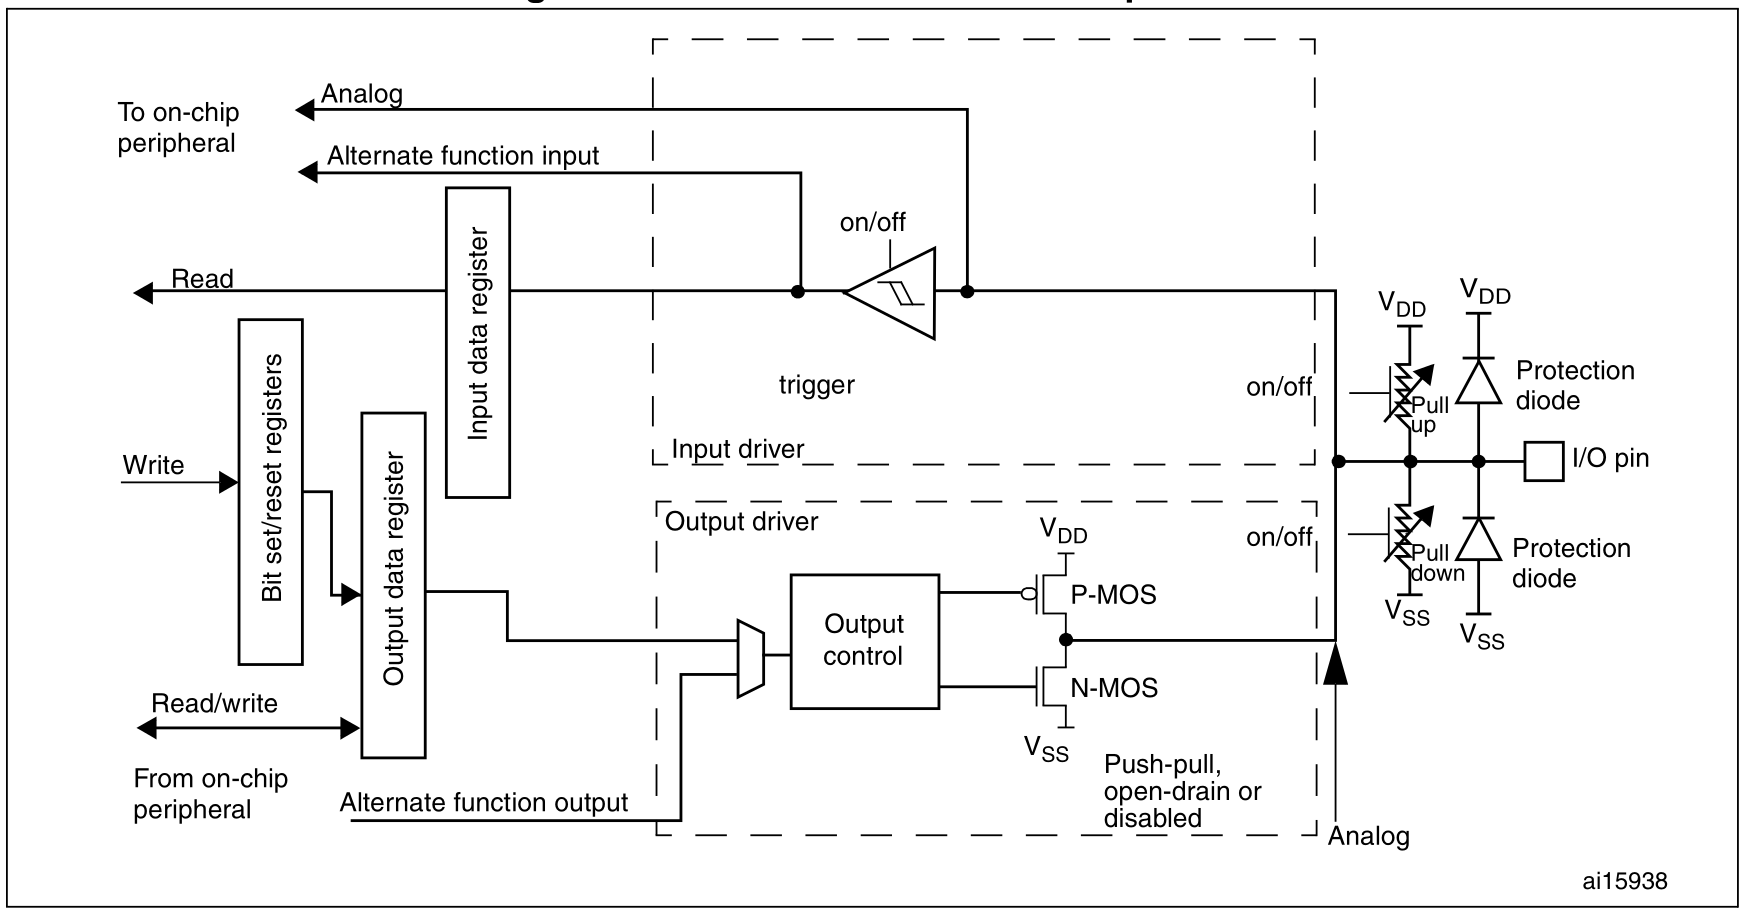
\includegraphics[width=0.9\linewidth]{support/pic/io_port.png}
\caption{Basic structure of an I/O port bit \cite{f303_ref}} %TODO citace - referencak F303
\label{fig:gpio}
\end{figure}

	\subsection{Timers}
	\label{sub:timers}
Timers are one of the basic peripherals. The primary function is counting; it can measure time and do a specific action, for example, toggle a pin. The counter clock frequency is adjustable using a programmable prescaler. Usually, there are many timers in the microcontroller with varying features.

The simplest ones are basic timers. These timers are predominantly used for time-base generation as they feature only a simple up counter, usually 16-bit.

The more feature-rich timers are general-purpose timers. With those, besides the basic functionality, it is possible to generate various waveforms or measure the pulse length of the input signal. Furthermore, there can be support for incremental encoders with quadrature output, which can then be connected straight to the MCU. This feature is handy and makes interfacing encoders pretty straightforward.

As the name suggests, the advanced-control timers are the most advanced. Functionality includes all the features of previously mentioned timers with some added or upgraded. Most of the time, advanced-control timers have more channels that can be synchronized together or using an external signal. This ability makes it possible to generate a three-phase PWM output to control a three-phase motor like BLDC.

The Cortex core contains another 24-bit timer called SysTick timer, dedicated to real-time operating systems. It usually provides OS with regular timer interrupts for time-keeping, but it can also be used as a standard down counting timer.

	\subsection{Analog-to-Digital Converter (ADC)}
	\label{sub:adc}
Another common peripheral is the Analog-to-Digital converter. This peripheral can convert a given voltage (usually between 0V and analog-reference voltage) to a binary number. One possible utilization can be reading a potentiometer voltage to obtain the trigger position.

The particular implementation can vary between the STM32 series, but most of the time, they use successive-approximation ADC or Sigma-Delta ADC. It can be configured to measure either single-ended input or differential input in continuous or single-shot mode. Also, some internal channels are available, for example, connected to an internal temperature sensor and voltage reference.

An internal ADC self-calibration is a convenient feature that can compensate for offset and gain error and significantly improve conversion accuracy. The calibration is triggered by software. If the application has to handle a large amount of data, the DMA unit can serve the ADC memory transfers to free the CPU. Moreover, an analog watchdog feature can monitor the converted voltage and generate an interrupt if it exceeds the programmed thresholds. 

	\subsection{Digital-to-Analog Converter (DAC)}
	\label{sub:dac}
The Digital-to-Analog converter does the exact opposite of the Analog-to-Digital converter. It converts the given binary number to a corresponding analog voltage. It is possible to generate complex waveforms or an audio signal with this peripheral. The DAC can therefore be used in many audio applications. If at least two channels are available, the conversion can be independent or simultaneous with external triggers, providing the ability to generate a stereo audio signal. Usually, the DAC also features a noise-wave generation or a triangular-wave generation. Such as with the ADC, the DAC memory transfers can be controlled by DMA, thus freeing up the CPU.

	\subsection{Serial Peripheral Interface (SPI)}
	\label{sub:spi}
The serial peripheral interface is a master-slave interface bus used to communicate with smaller devices, such as sensors, memories, displays, or LED drivers. If supported by a particular microcontroller, the peripheral can also be configured as an I2S (Inter-Integrated Sound) interface, allowing the connection of digital audio devices.

Peripheral settings are rich to support a wide range of compatible devices. It can operate either as a master, providing a clock to connected devices, or as a slave; multimaster mode is also possible. Communication mode and speed can be configured as well as frame size and clock polarity. The DMA unit can help handle a lot of data and achieve high data communication rates with hardware control. Moreover, the SPI peripheral includes a hardware CRC unit with automatic CRC error checking. This feature can be helpful when communicating with SD memory cards.

	\subsection{Inter-Integrated Circuit (I2C)}
	\label{sub:i2c}
The Inter-Integrated Circuit is another commonly used short-range communication bus in embedded systems. It is also a synchronous interface that requires fewer communication wires than SPI but provides lower communication rates. As the SPI interface, the I2C can be used to communicate with small displays, memories, and other rather lower-speed devices.

The peripheral supports both 7-bit and 10-bit addressing modes, programmable analog and digital noise filters, and configurable multiple speed modes depending on the particular microcontroller. Furthermore, the peripheral includes a hardware CRC unit, and it is designed to support SMBus and PMBus protocols used by PCs and servers. DMA channel connecting I2C is also available to provide hardware control of transfers.

	\subsection{USART}
	\label{sub:usart}
USART stands for Universal Synchronous/Asynchronous Receiver/Transmitter. Although computers are rarely equipped with serial ports these days, serial communication is still highly used in the embedded world as it is simple and easy to use. This peripheral is flexible and has a wide range of applications - it can be used for simple UART communication; in the synchronous mode, it can act like SPI master/slave; it also features hardware management of some signals from industry standards like RS-232 and RS-485. Moreover, there is support for Smartcard communication, IrDA serial infrared communication, and multiprocessor communication. It is also possible to use the peripheral to implement other buses with hardware control, for example, Modbus or 1-Wire.  

The peripheral offers many programmable parameters like baud rate, data word length, the number of stop bits, data order, parity control, or oversampling. Furthermore, USART is the source of many interrupts indicating various statuses and flags. The peripheral is connected to the DMA unit like other serial communication peripherals, significantly facilitating the handling of continuous streams or huge amounts of data.

%!TEX ROOT=slehokri_bp.tex


\part{Hardware}
\label{chap:hw}
%\section{Indroduction}
%\label{sec:hw_intro}


\section{Chassis and transmitter}
\label{sec:hw_base}
\subsection{Background}
The whole project is built on an old entry-level onroad 1/10 chassis from the Tamiya Quick Drive series released on Jul 16, 2003 [\todo citace]. The RC car was obtained as a childhood gift. It was pre-assembled and came with a 2-channel transmitter communicating at a frequency of \SI{27}{\MHz}. Later the servo broke, and no repair or upgrade parts were available. Since the repair was nearly impossible, but the rest of the chassis was fully functional, it was the perfect choice for a complete rebuild.

The car featured a sealed gearbox, servo, "280" size brushed motor and \SI{9.6}{\V} Ni-Cd battery pack. Due to the age of the product, not much technical information can be found.

\subsection{Modifications}
\label{sec:hw_mods}
All the electronics were removed, leaving only the plastic chassis. The broken 5-wire servo was replaced with a "standard" size hobby servo used in most 1/10 RC cars [\todo info]. The old brushed motor was still functional, but it was decided to replace it with a newer and more powerful one. The only constraint was a shaft size, as the old pinion had to be transferred to the new motor to maintain functionality. Therefore a "2435" size BLDC motor with a \SI{25}{\A} ESC was selected. More information about the servo and BLDC is in sections \ref{sec:hw_servo} and \ref{sec:hw_bldc}. Furthermore, the plastic bearings were replaced by metal ball bearings.

A 2-cell LiPo battery with a capacity of \SI{2200}{\milli\A\hour} was chosen to supply power to the electronics. According to the product specification, this battery should withstand 35C of continuous current [\todo citace]. The term "35C" means "35 times the battery capacity". For this particular battery, that means $35 \cdot \SI{2.2}{\A} = \SI{77}{\A}$ of current, which is more than sufficient.

The transmitter underwent a similar procedure. The original circuit board and the antenna were also removed, retaining only trigger potentiometers and plastic parts. Potentiometers used for throttle and steering trimming were replaced with rotary encoders. Again, the power supply is a 2-cell LiPo battery with a lower capacity of only \SI{900}{\milli\A\hour} and 25C of continuous current.



\section{Servo}
\label{sec:hw_servo}
A servomotor, or servo for short, is an actuator used for precise output shaft positioning. It consists of a motor with position feedback and a control board. RC servos are controlled using a 50Hz PWM signal. The output angle is linearly dependent on a pulse width between \SI{1}{\ms} and \SI{2}{\ms}. The diagram in figure \ref{fig:servo_control} illustrates typical timing.
\begin{figure}[t]
\centering
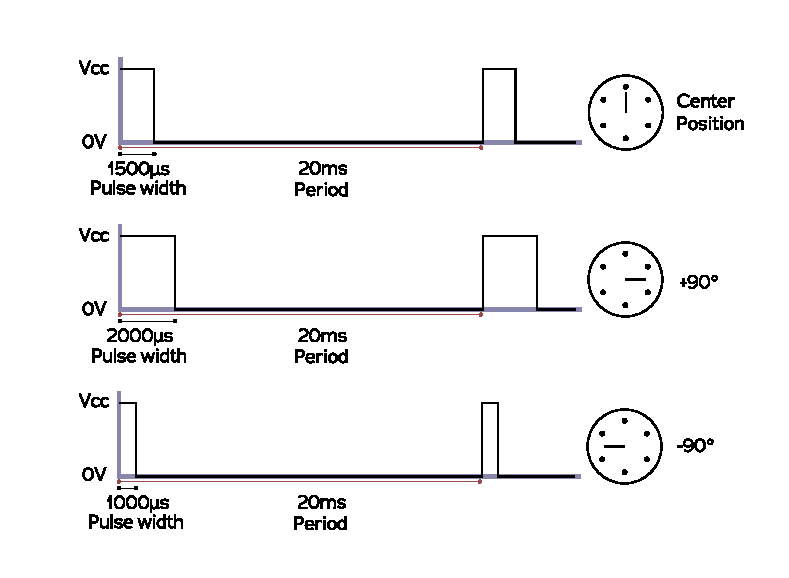
\includegraphics[width=0.7\linewidth]{fig/Servomotor_Timing_Diagram.pdf}
\caption{Servomotor timing diagram \cite{servo_control}}
\label{fig:servo_control}
\end{figure}

The servo used in the car is TowerPro MG995. It has metal gears and operating voltage between \SI{4.8}{\V} to \SI{6.6}{\V}. Speed and torque depend on the supply voltage. According to the product specifications [\todo citace], the servo can achieve operating speed of $0.2\, \text{s}/60^\circ$ and torque of \SI{9.4}{\kg\per\cm} with the \SI{4.8}{\V} supply voltage. From the operating speed we can calculate angular velocity: 
\begin{equation}
\omega = \frac{d \theta}{d t} = \frac{\frac{\pi}{3}}{0.2} \doteq 5.236\ \unit{\radian\per\second}\ .
\end{equation}
Since the servo supply voltage is \SI{5}{\V}, both speed and torque values should be slightly higher.


\section{Motor and ESC}
\label{sec:hw_bldc}
As mentioned in section \ref{sec:hw_mods}, the biggest BLDC with a shaft diameter of \SI{2}{\mm} was selected to replace the old brushed one. The motor was supplied in a set including a \SI{25}{\A} Electronic Speed Controller (ESC). The type is GoolRC 2435 \SI{4800}{\Kv}\footnote{\unit{Kv} refers to rpm/min/V with no load attached to the motor} BLDC; available information about the motor is in table \ref{tab:BLDC_spec} and about ESC in table \ref{tab:ESC_spec}. Since the BLDC motor is directly connected to the ESC and the car communicates only with the ESC, the BLDC is considered a black box.

RC ESCs are controlled the same way as RC servos; thus, the same timing diagram in figure \ref{fig:servo_control} applies. The only difference is the resulting motion. Pulse width with a duration of \SI{2}{\ms} equals full forward acceleration, pulse width with a duration of \SI{1.5}{\ms} equals neutral, and pulse width with a duration of \SI{1}{\ms} equals full brake/reverse.

Whether the brake or reverse is activated depends on the actual motion of the motor. If the car is going forward (meaning the motor rotates forward) and the pulse width becomes lower than \SI{1.5}{\ms}, first, the brake is activated and remains activated until the pulse width is again \SI{1.5}{\ms} or greater. The car must be almost static to start reversing; otherwise, the ESC will stay in brake mode. If the car is static or is already reversing, a pulse width lower than \SI{1.5}{\ms} activates reverse mode.

\begin{table}[t]
   %\renewcommand{\arraystretch}{1.1}
   \tabcolsep 18pt
   \centering
    \caption{BLDC specifications}\label{tab:BLDC_spec}   
    \begin{tabular}{l r}
       \noalign{\hrule height 1.1pt}\noalign{\smallskip}	   
	Power			& 300\unit{\W}\\
	Max. voltage   	& 12.6\unit{\V}\\
	Max. current   	& 24\unit{\A}\\
	Rotor poles	   	& 4 \\
	\unit{\Kv} rating	  	& 4800 \\
	Length			& 24\unit{\mm} \\
	Diameter			& 35\unit{\mm} \\
	Shaft diameter	& 2\unit{\mm} \\
       \noalign{\smallskip}\noalign{\hrule height 1.1pt}
    \end{tabular}
\end{table} 
\begin{table}[t]
   %\renewcommand{\arraystretch}{1.1}
   \tabcolsep 12pt
   \centering
    \caption{ESC specifications}\label{tab:ESC_spec} 
    \begin{tabular}{l r}
       \noalign{\hrule height 1.1pt}\noalign{\smallskip}
	Continuous current		& 25\unit{\A}\\
	Instantaneous current   	& 50\unit{\A}\\
	BEC type				   	& 5\unit{\V}, 2\unit{\A}\\
	Battery				   	& 2-3 Cell LiPo \\
       \noalign{\smallskip}\noalign{\hrule height 1.1pt}
    \end{tabular}
\end{table} 

\section{Control board}
\label{sec:hw_control}
Prototyping was mainly done on the breadboard using the RobotDyn's BlackPill development board featuring STM32F303CCT6 microcontroller \cite{black_pill}. The board uses a similar size and form factor as the popular BluePill board equipped with STM32F103C8T6 \cite{blue_pill}. Both these boards were readily available. BlackPill was selected for its better processor based on an ARM M4 core with FPU, larger memories, and more advanced peripherals. The board is shown in figure \ref{fig:black_pill}.
\begin{figure}[t]
\centering
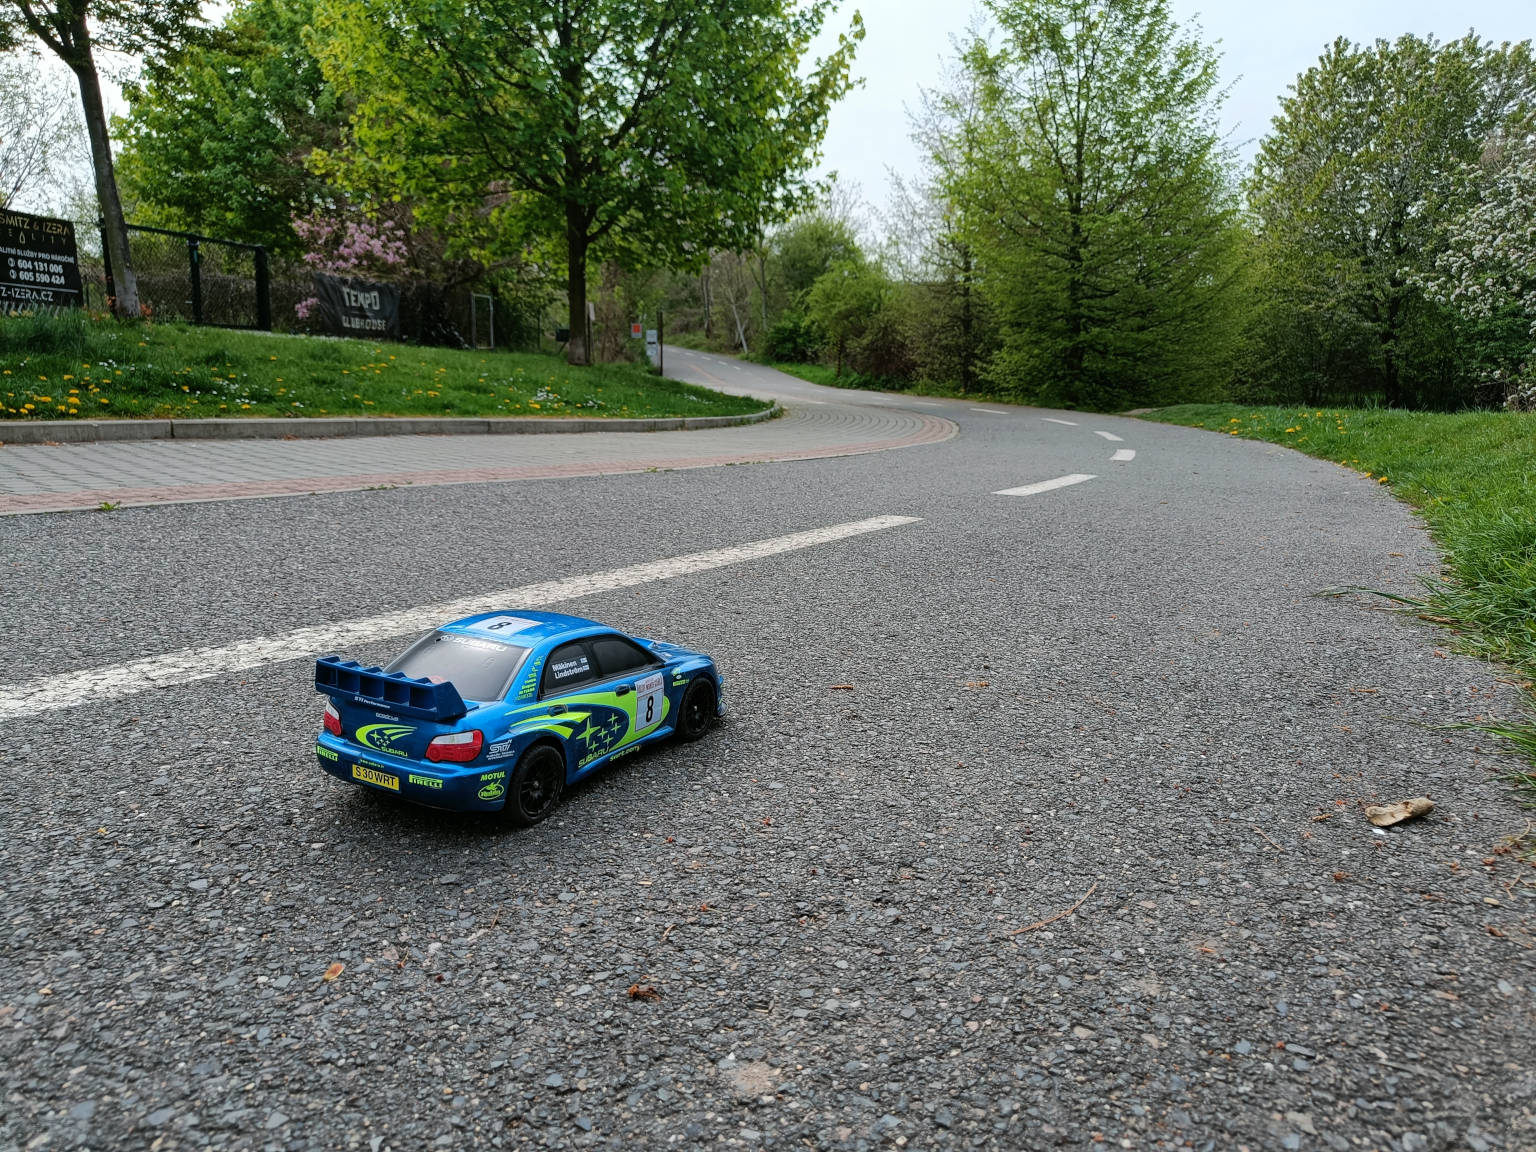
\includegraphics[width=0.5\linewidth]{support/pic/placeholder.jpg}
\caption{*PLACEHOLDER* RobotDyn BlackPill development board}
\label{fig:black_pill}
\end{figure}


\section{Communication}
\label{sec:hw_comm}
The project uses wireless modules equipped with nRF24L01+ transceiver chip from Nordic Semiconductor [\todo citace], a power amplifier, a low-noise amplifier, and an external antenna. The chip operates in the worldwide \SI{2.4}{\GHz} ISM band and communicates with the MCU using the SPI bus. Configurable parameters include channel, data rate, and output power. These modules fit all the requirements, and in addition, they are cheap and readily available.

According to the product specification [\todo cit-Amazon], the range should be more than \SI{800}{\m} line-of-sight. Thanks to the Enhanced ShockBurst protocol and its Auto Acknowledgement function [\todo citace], attaching a small payload to the ACK packet is possible. This feature is advantageously used to report car status back to the transmitter.


\section{Sensors}
\label{hw_sensors}
In addition to measuring the voltage, which is necessary for battery monitoring and is realized using a voltage divider, the car also measures current and BLDC case temperature. It is also equipped with 6-axis IMU. In the project's present state, data from sensors are mainly informative and are not used for control purposes.

The transmitter does not use any particular sensor; only battery voltage is measured.

\subsection{Current}
The current is measured using a module with a 30A version of an ACS712 chip. It is a small linear current sensor based on the Hall effect. Current flowing through the sensor's copper terminals generates a magnetic field, which is then sensed by the integrated Hall-effect circuit. The output of the sensor is a voltage proportional to the flowing current. Current sense terminals are electrically isolated from the rest of the sensor; therefore, it is possible to measure high voltages without external electrical isolation. The sensor is capable of measuring both AC and DC current with a stated total output error of $1.5\%$ [\todo citace]. 

\subsection{Temperature}
A digital thermometer DS18B20 provides temperature measurement. The sensor is manufactured by Dallas Semiconductor, which Maxim Integrated later acquired. It can measure temperatures from \SI{-55}{\degreeCelsius} to \SI{125}{\degreeCelsius}. It has a programmable resolution ranging from 9 to 12 bit and $\pm$\SI{0.5}{\degreeCelsius} over most of the measuring range. The sensor uses a 1-Wire interface, which requires only one pin for communication. When combined with parasitic power mode, the whole thermometer requires only two pins for operation [\todo citace].

The project uses the TO-92 package, which was advantageous because of the limited space around the BLDC. The small size made it possible to mount the sensor on the back of the motor housing with the aid of heat-conducting foil.

\subsection{IMU}


\section{Status info}
\label{hw_status}
Neither the RC car nor the transmitter reported any status in the original version. The user had to check the battery state himself; otherwise, the battery could be discharged entirely and damaged. Since LiPo batteries should not be discharged below a certain threshold, the usual rule of thumb across the RC community is not to discharge the battery below \SI{3.1}{\V} per cell, it was necessary to report the battery status.

An RGB LED was chosen for that purpose because it is possible to quickly report the various states to the user using different colors. On the other hand, it is unsuitable for visualizing values such as temperature. Besides, the transmitter has its own battery, whose status should also be reported to the user, and that would need 2 LEDs. The single RGB LED was therefore insufficient for the transmitter.

For this reason, the display seemed like a good alternative and replacement. An OLED display was convenient as its power consumption is low, it is readable in direct sunlight, and thanks to only one color, it is fast. The disadvantage is its small size, which complicates the orientation in the displayed data.

Considering all the factors, both the RGB LED and the OLED display were used. RGB LED serves as a fast state notifier, and further status information can be found on the display.

Both car and transmitter use RGB LED with a common anode and monochrome OLED display module with SSD1306 chip communicating using I\textsuperscript{2}C bus [\todo citace].


%\begin{table}[t]
%\centering
%\caption{*PLACEHOLDER* BLDC specifications} %TODO citace
%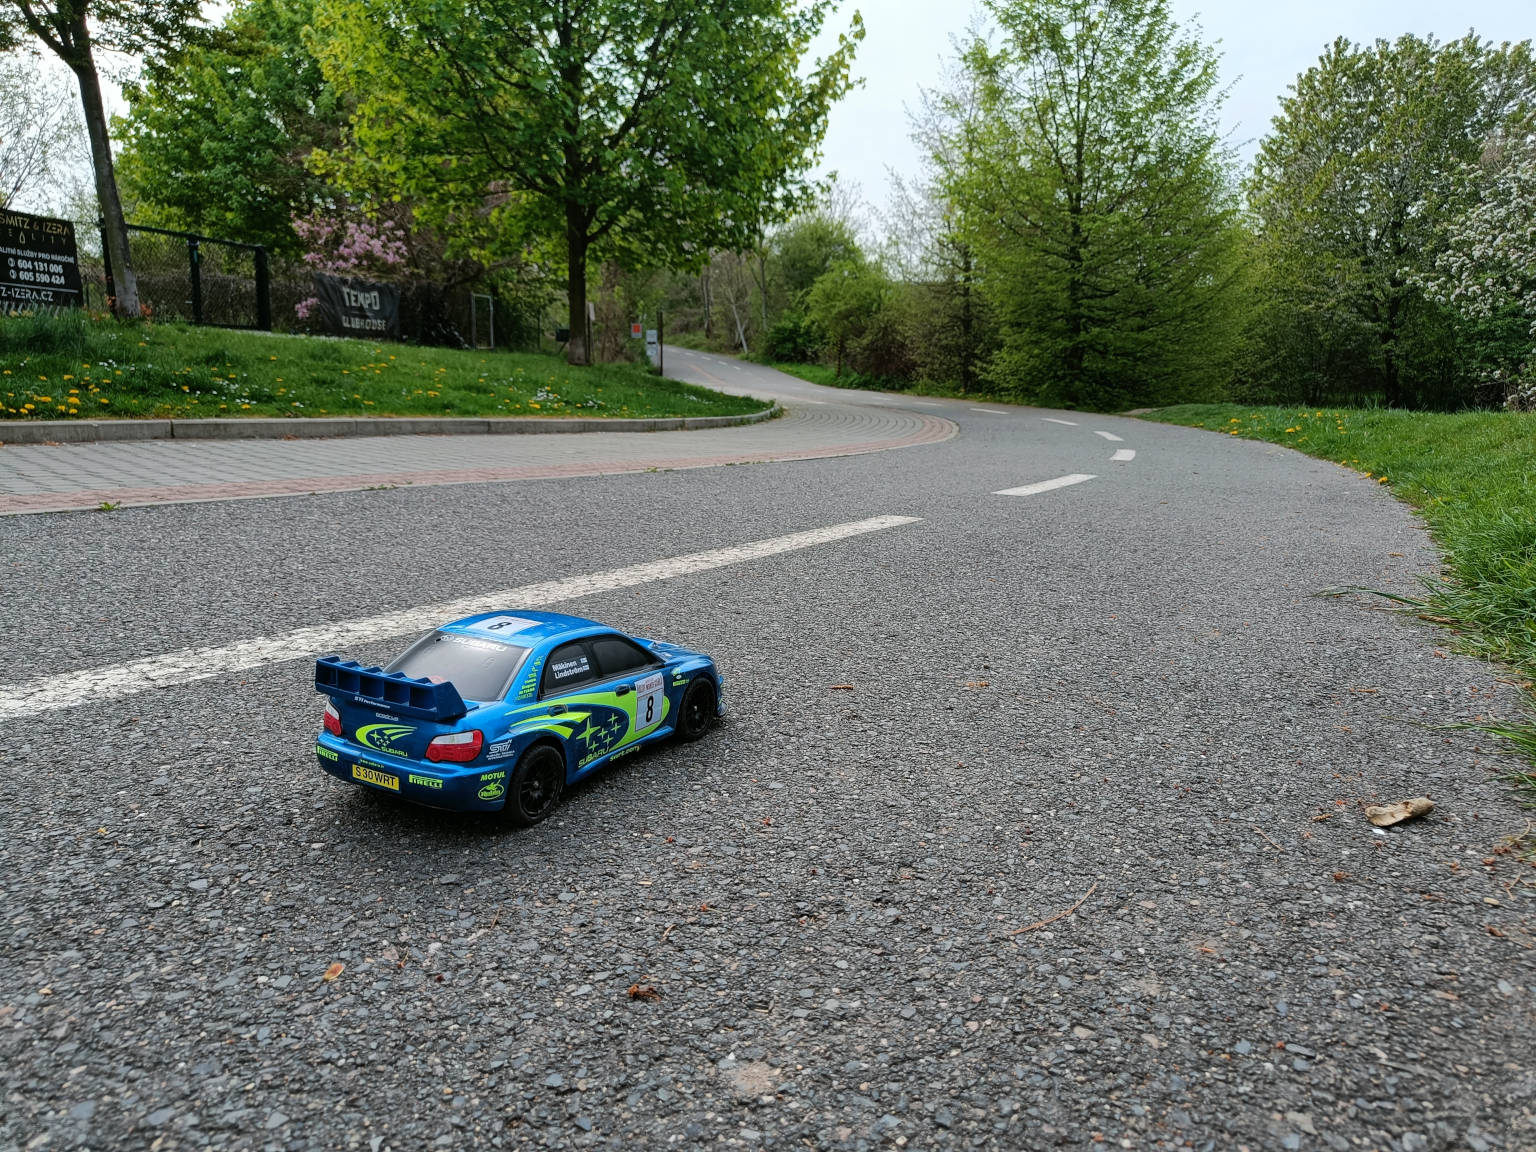
\includegraphics[width=0.8\linewidth]{support/pic/placeholder.jpg}
%\label{tab:BLDC_spec}
%\end{table}






\nocite{*}
\bibliographystyle{unsrt}
\bibliography{slehokri_bib}					%TODO
%\ctutemplate{specification.as.chapter}		%TODO








\end{document}
